\section{Resultados e Discussão}

A PIRNN apresentou previsões altamente consistentes com a simulação de referência realizada pelo \textit{CasADi} com o método RK4. A Figura \ref{fig:pirnn-results} ilustra os resultados da validação, evidenciando que a PIRNN conseguiu reproduzir com elevada fidelidade a dinâmica do sistema mesmo ao aplicar intensas perturbações na vazão de entrada durante aproximadamente 33 horas de operação.

\begin{figure}[ht]
  \centering
  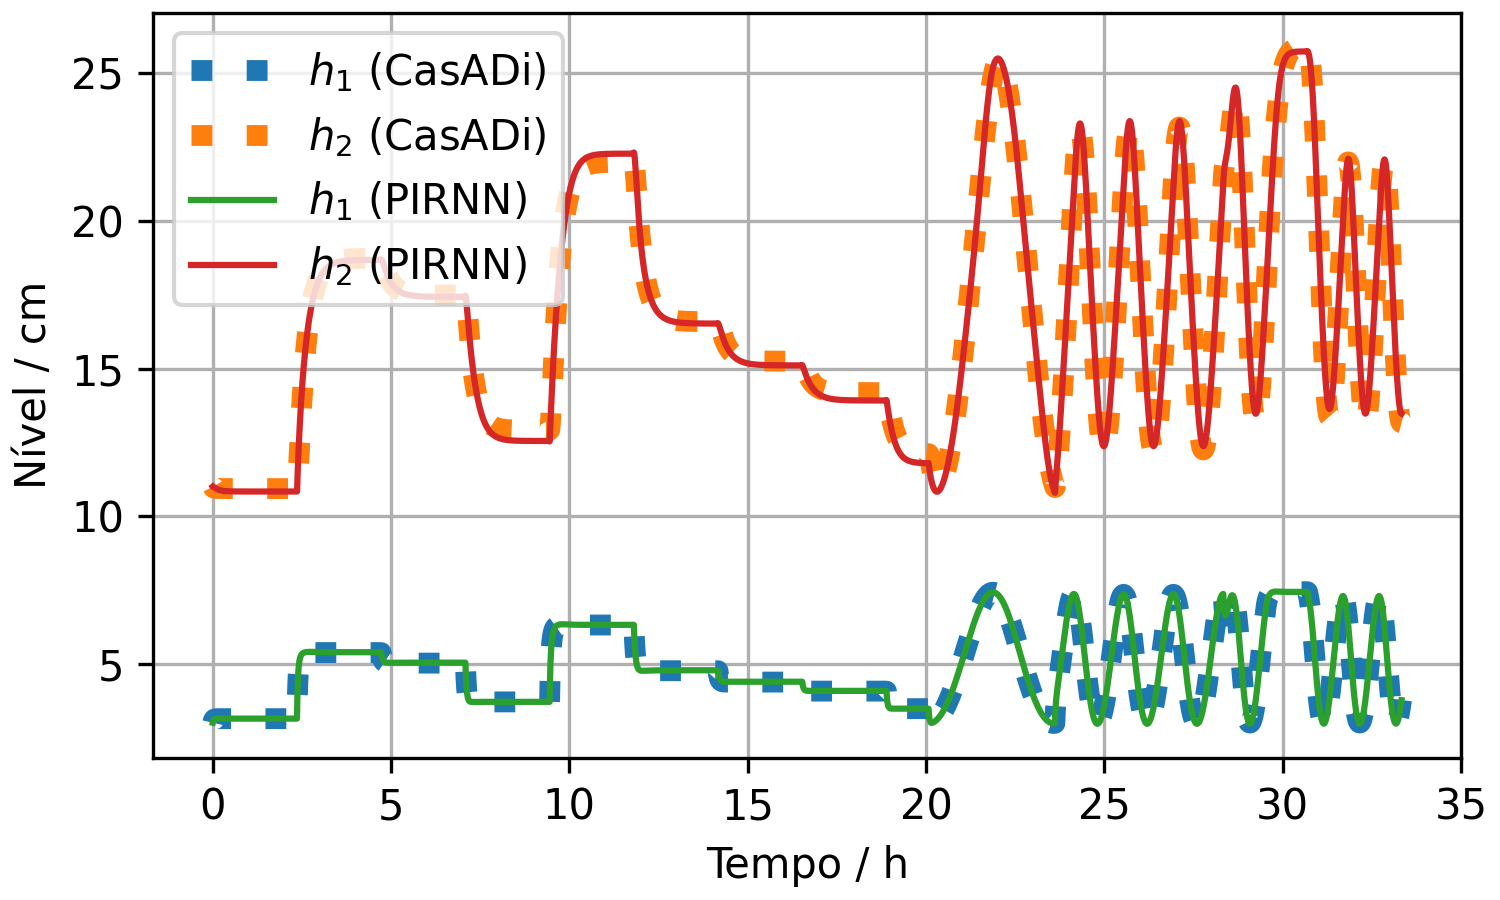
\includegraphics[width=0.45\textwidth]{pirnn-test.png}
  \caption{Comparação entre as previsões da PIRNN e o modelo de referência simulado no \textit{CasADi}.}
  \label{fig:pirnn-results}
\end{figure}

A implementação da PIRNN no Arduino demonstrou um uso eficiente dos recursos computacionais: verificou-se que o programa completo, que inclui a PIRNN, o controlador PI e o código responsável pela comunicação serial com o computador, utilizou 69,1\% da memória flash e apenas 15,9\% da memória RAM do Arduino. Esses números indicam que existem recursos disponíveis para implementação de modelos mais complexos ou execução de tarefas adicionais, caso necessário.

\begin{figure}[ht]
  \centering
  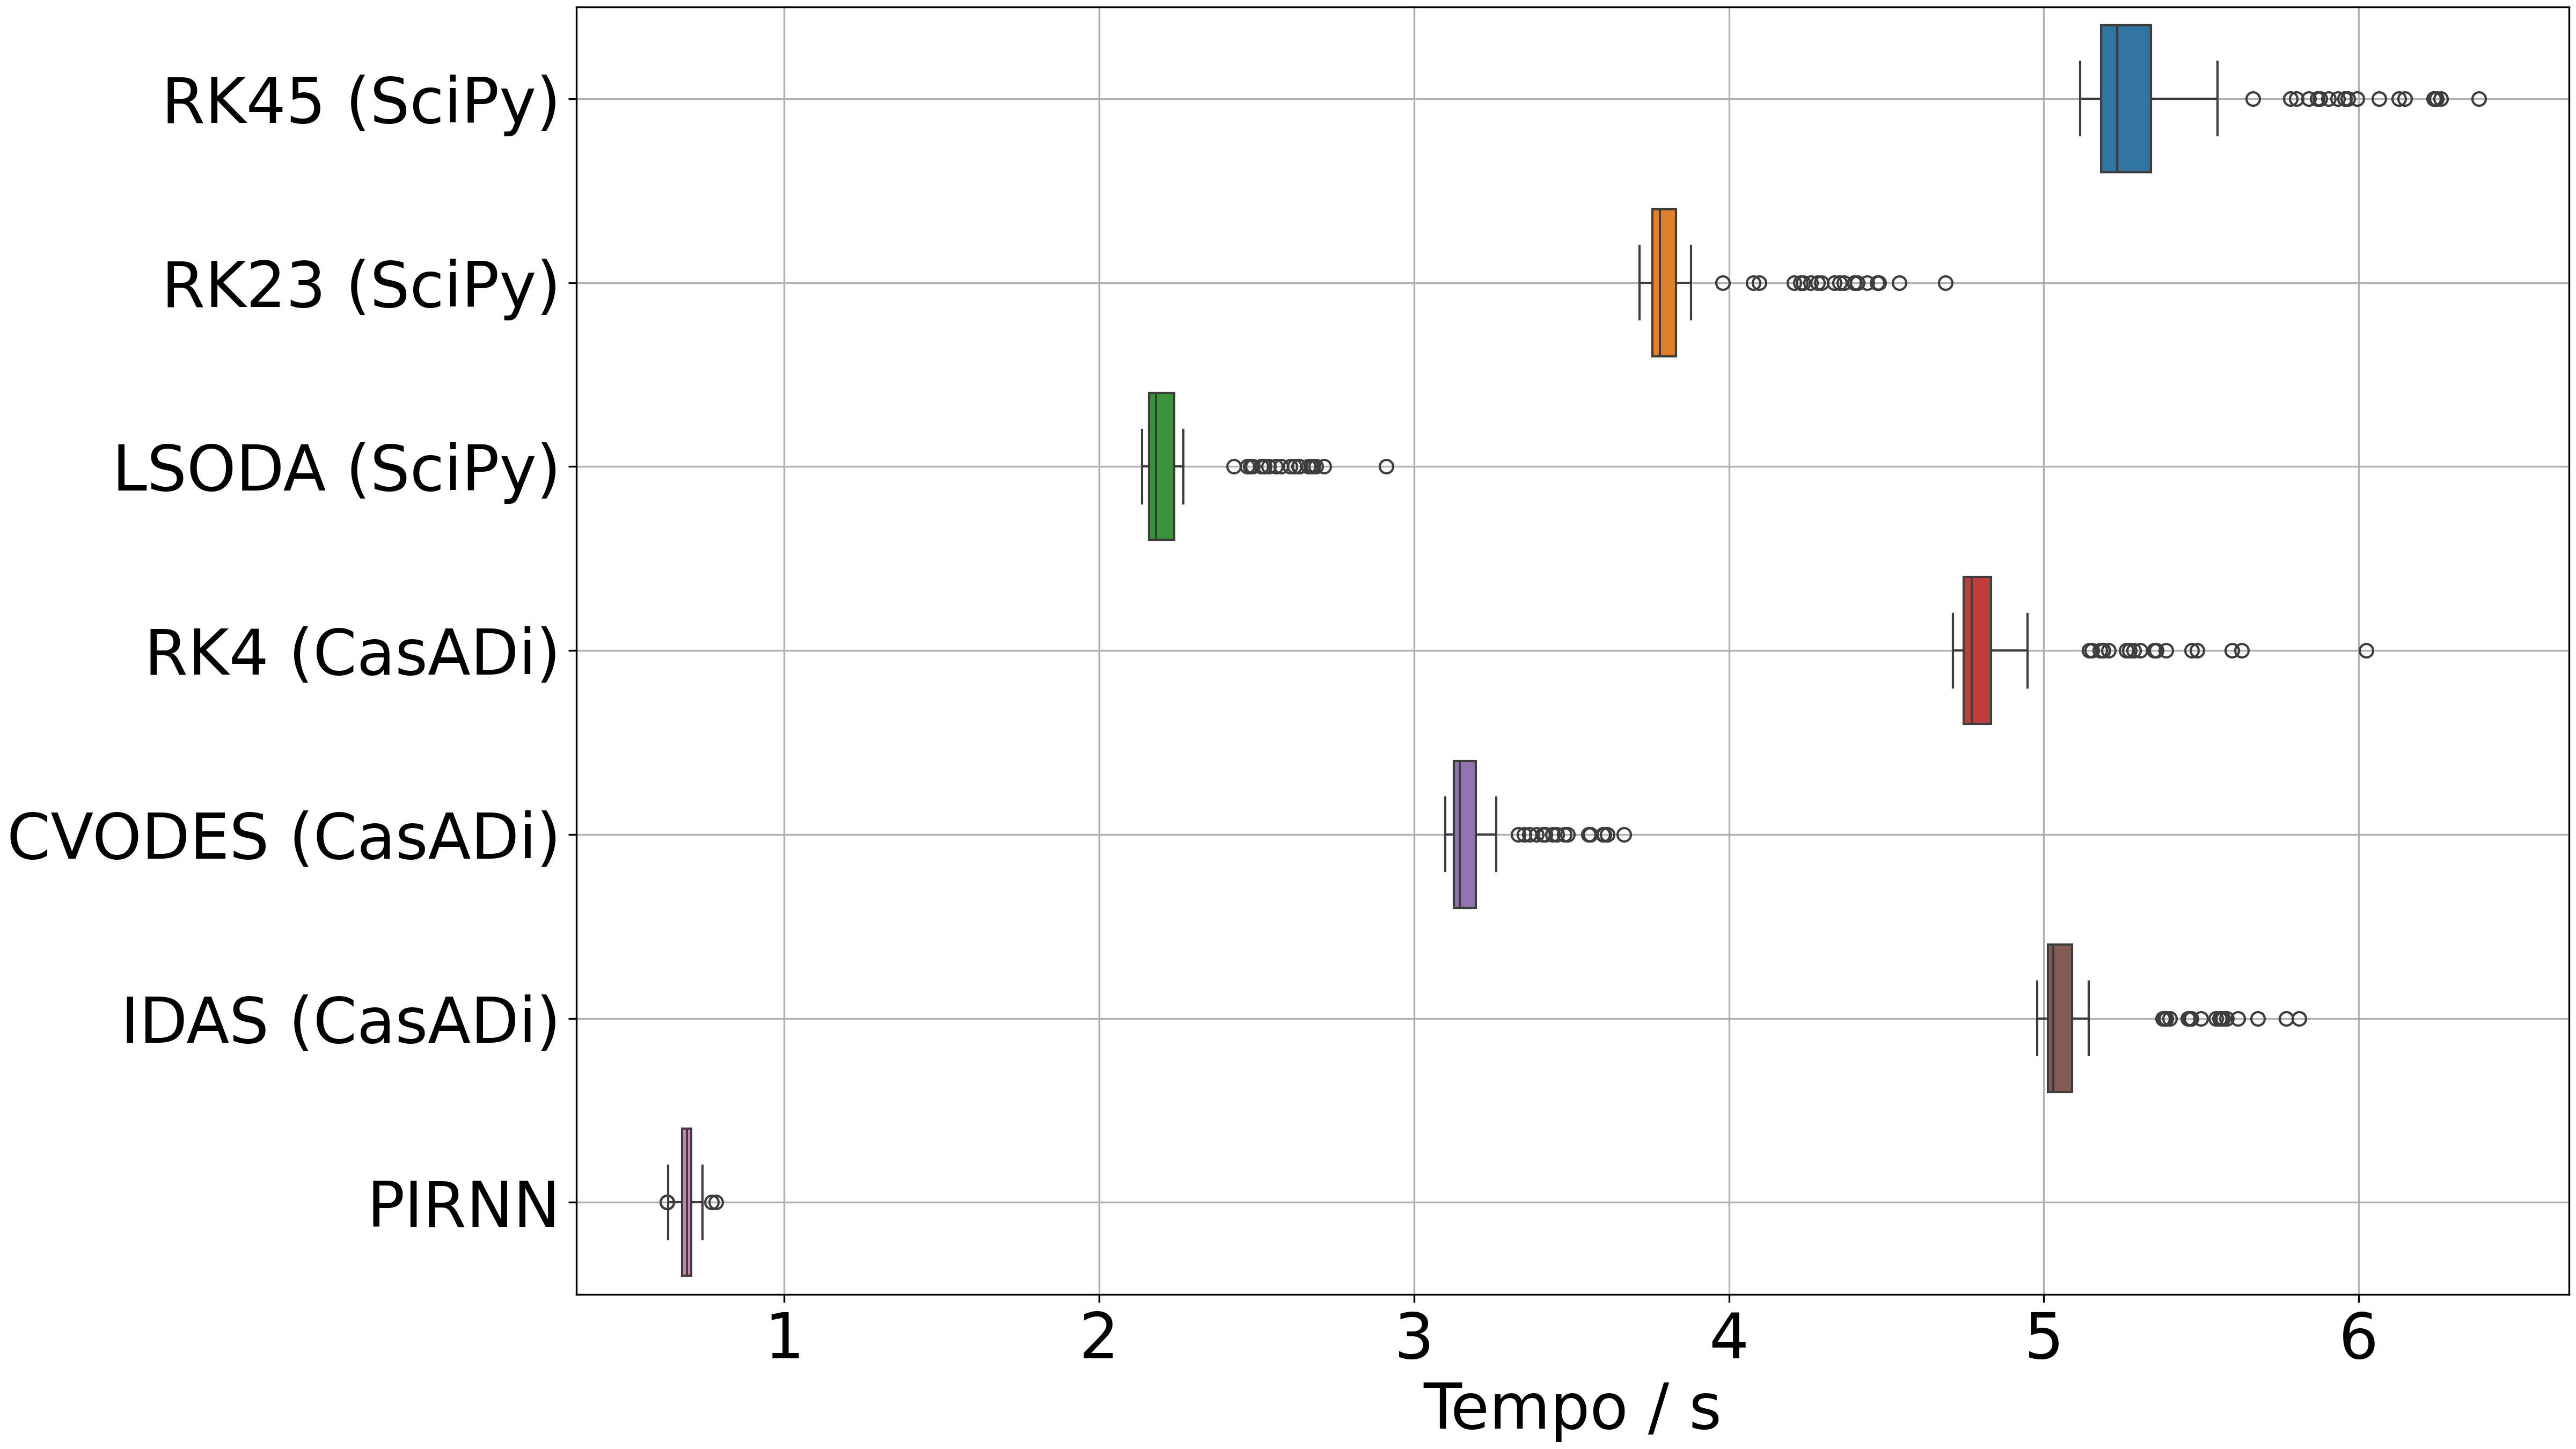
\includegraphics[width=0.45\textwidth]{pirnn-boxplot.png}
  \caption{Boxplot dos tempos de execução dos métodos avaliados.}
  \label{fig:pirnn-benchmark-lite}
\end{figure}

\begin{figure*}[ht]
  \centering
  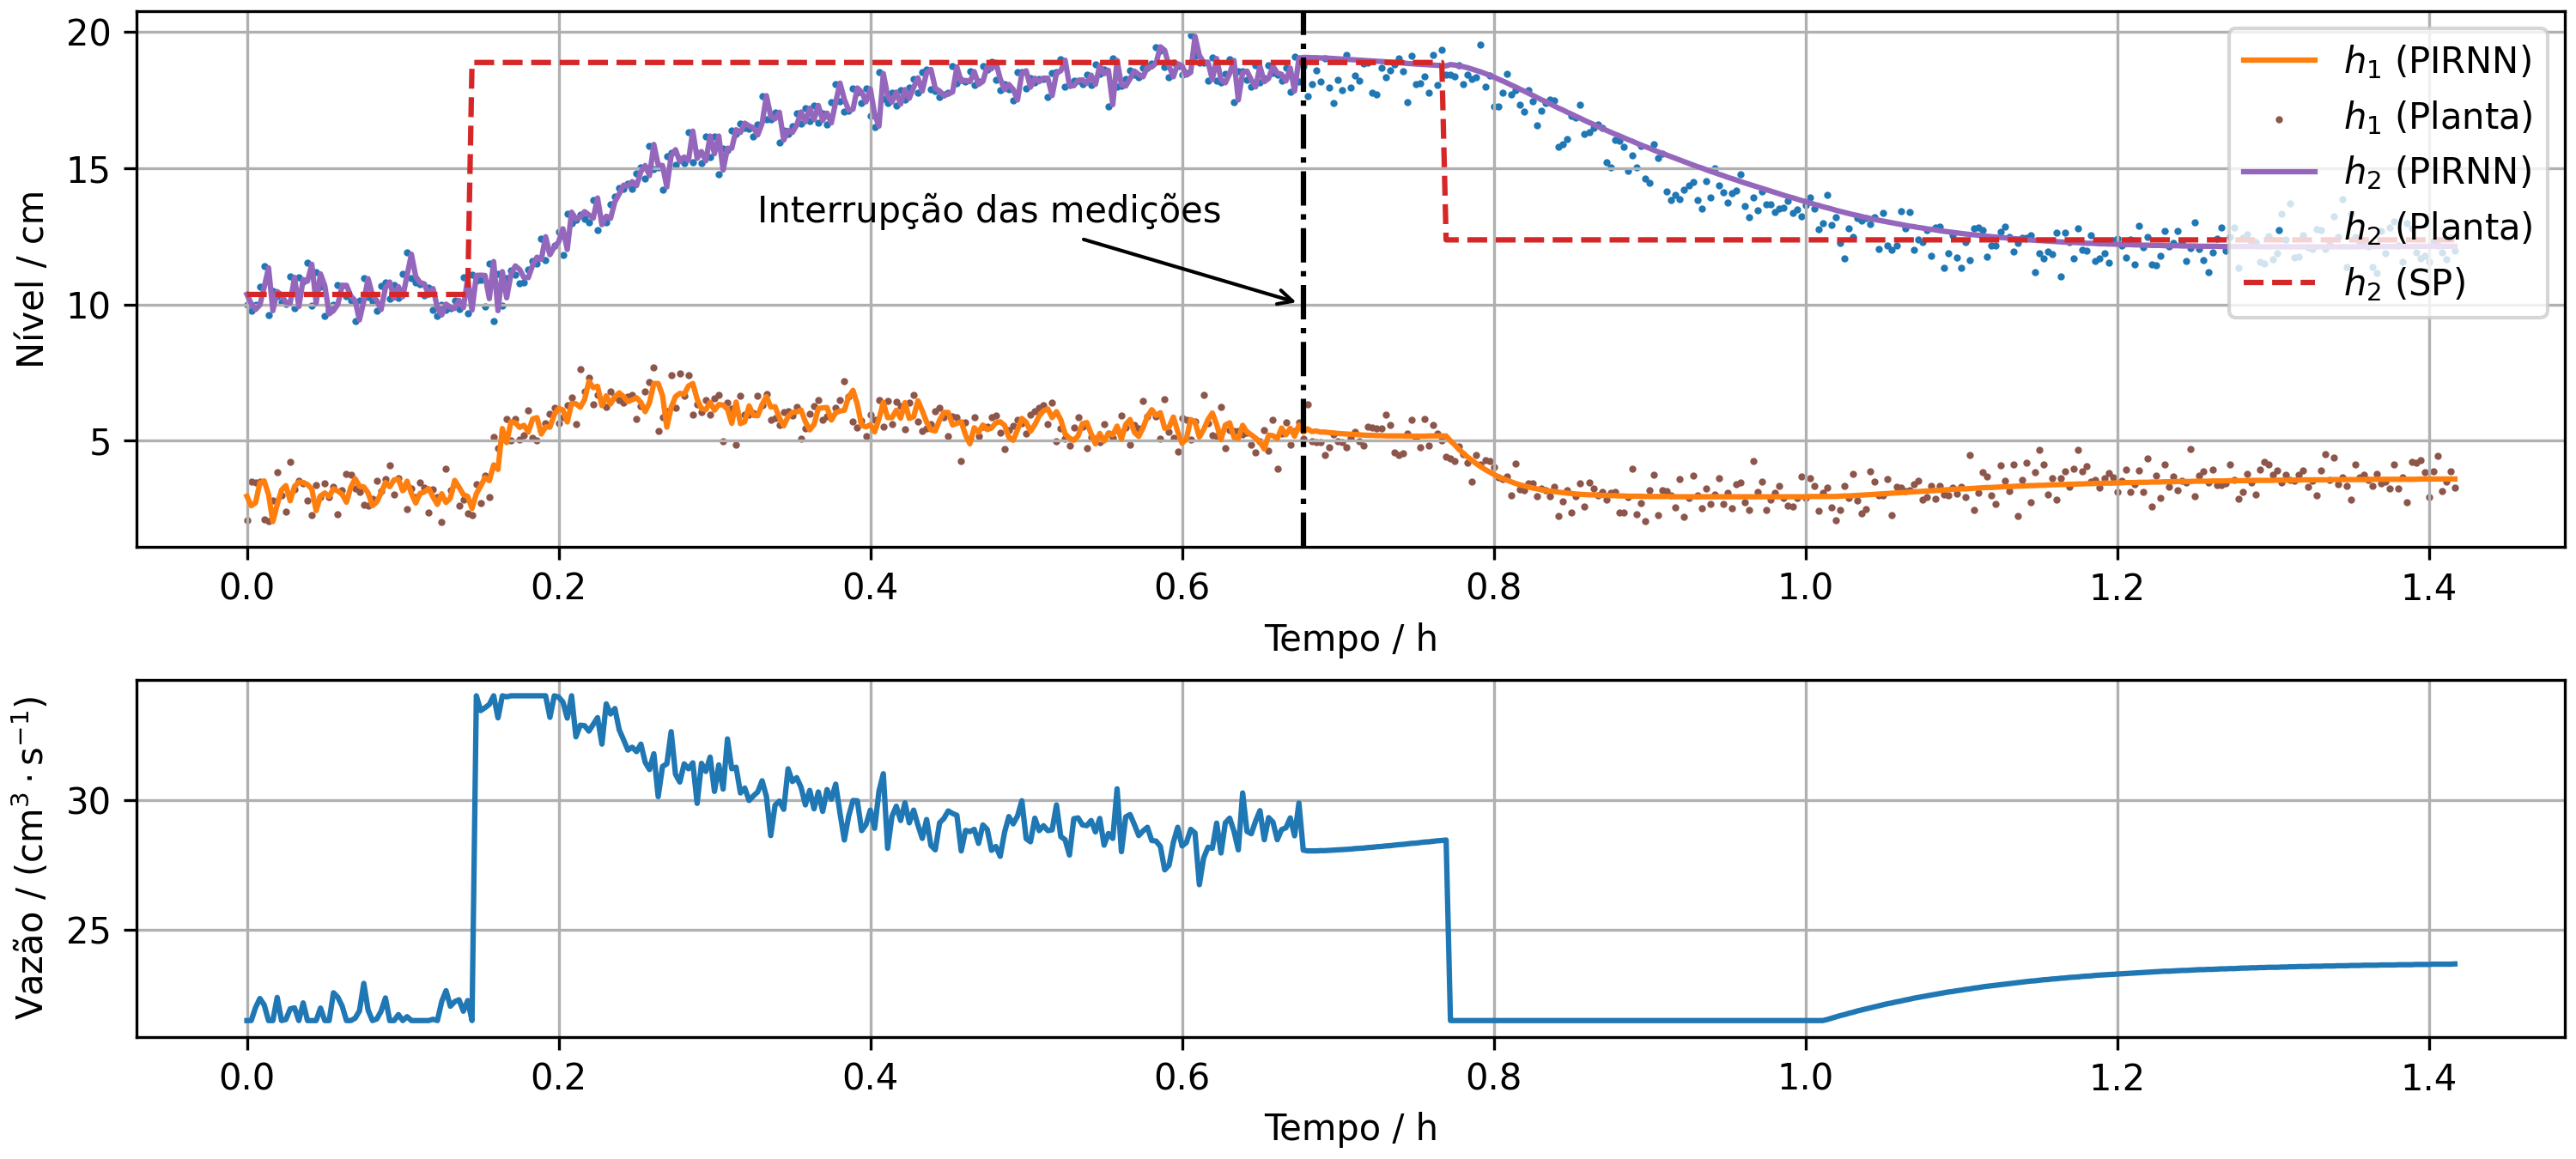
\includegraphics[width=0.8\textwidth]{hil-pirnn-pi.png}
  \caption{Comparação entre as leituras dos sensores, obtidas a partir dos níveis simulados com adição de ruído, e os níveis previstos pela PIRNN embarcada após uma perturbação do tipo degrau na vazão de entrada. A linha preta ponto-traço vertical indica o instante em que os valores dos sensores deixam de ser enviados ao Arduino, fazendo com que a PIRNN passe a se retroalimentar.}
  \label{fig:sil-pirnn}
\end{figure*}

Nos testes de desempenho, a PIRNN demonstrou uma significativa vantagem em termos de velocidade quando comparada com métodos numéricos tradicionais. A comparação foi feita com a implementação dos métodos RK4, CVODES e IDAS da biblioteca \textit{CasADi}, e dos métodos Runge-Kutta de quinta ordem com estimativa de erro de quarta ordem (RK45), Runge-Kutta de terceira ordem com estimativa de erro de segunda ordem (RK23) e LSODA da biblioteca \textit{SciPy}, todos executados no mesmo computador. Para avaliar o desempenho de cada método, foram realizadas 100 execuções de cada algoritmo sob as mesmas condições de entrada utilizadas na validação. A Figura \ref{fig:pirnn-benchmark-lite} apresenta o boxplot dos tempos de cômputo dos métodos avaliados, evidenciando a superioridade da PIRNN em termos de tempo de processamento.

% Local original da imagem pirnn-benchmark-lite

Nos testes de robustez, foram simulados cenários com ruído nas medições e com ausência completa de medições. A Figura \ref{fig:sil-pirnn} apresenta os resultados obtidos nesses testes. Observa-se que no caso de medições ruidosas, a PIRNN capta as variações geradas pelo ruído, mas com um leve amortecimento, sugerindo uma capacidade de filtragem parcial das perturbações. Quando as medições são interrompidas completamente, a PIRNN passa a se retroalimentar. Nesse cenário, ela continua seguindo com precisão o comportamento esperado dos tanques, mesmo sem a entrada de dados dos sensores. Vale destacar que, mesmo nessas condições adversas, o controlador PI implementado no Arduino continua atuando corretamente no sistema, alcançando o \textit{setpoint} com base apenas nas informações fornecidas pela PIRNN.

% Local original da imagem fig:sil-pirnn